\documentclass[12pt]{article}

\usepackage{amsmath}
\usepackage{graphicx}
\usepackage[margin=0.7in]{geometry}
\usepackage{float}
\usepackage{listings}
\usepackage[utf8]{inputenc}
\usepackage[parfill]{parskip}  

\begin{document}
\title{Schrödingerlikningen
\\ Prosjekt 2
\\ FYS3150}
\author{Ragnar Bruvoll \and Halvard Sutterud}
%\author{Halvard Sutterud}
\date{September 2017}
\maketitle{\begin{center}\end{center}}
\pagenumbering{gobble}
\thispagestyle{empty}

\begin{abstract}
    We study the cases of one and two electrons trapped in a harmonic oscillator. 

\end{abstract}
\newpage
\pagenumbering{arabic}


\section*{Abstract}
Ser på den radielle Schrôdringerligninen for ett elektron. Den ser slik ut:


\section*{Introduction}
Eigenvalues a


\section*{Theory/Methods}
\subsection*{Making the matrix}
The analytical Schroedringer equation is as follows
\begin{equation*}
  -\frac{\hbar^2}{2 m} \left ( \frac{1}{r^2} \frac{d}{dr} r^2
  \frac{d}{dr} - \frac{l (l + 1)}{r^2} \right )R(r) 
     + V(r) R(r) = E R(r)
\end{equation*}
where  $V(r) = (1/2)kr^2$ is the harmonic oscillator potential, k is the displacement factor where $k=m\omega^2$.
$\omega$ is the frequence of the oscillator and m is the mass of whatever's oscillating, in this case the electron. E is the energy og the oscillator and will take the values

\begin{equation*}
E_{nl}=  \hbar \omega \left(2n+l+\frac{3}{2}\right),
\end{equation*}

due to quantum mechanical effects, where n and l are quantum numbers with the following possible values $n=0,1,2,\dots$ and
$l=0,1,2,\dots$. R is the wave function, dependant on distance r. We'll be using spherical coordinates, such that $r\in [0,\infty)$ is the distance from the center of the oscillator to the position of the electron.\\

In order to simplify the equation, we'll make the new variable $u(r)$ such that $R(r) = (1/r) u(r)$. This gives

\begin{equation*}
  -\frac{\hbar^2}{2 m} \frac{d^2}{dr^2} u(r) + \left ( V(r) + \frac{l (l + 1)}{r^2}\frac{\hbar^2}{2 m}\right ) u(r)  = E u(r)
\end{equation*}

the next step in generalizing the equation will be making the variable dimentionless by introducing a new variable $\rho = (1/\alpha) r$ where  $u(0)=0$ and $u(\infty)=0$. The equation is now a function of the dimentionless $\rho$.

\begin{equation*}
  -\frac{\hbar^2}{2 m \alpha^2} \frac{d^2}{d\rho^2} u(\rho)+ \left ( V(\rho) + \frac{l (l + 1)}{\rho^2}\frac{\hbar^2}{2 m\alpha^2} \right ) u(\rho)  = E u(\rho)
\end{equation*}
We will be looking at a case with no angular momentum, $l=0$. The last step will be inserting the potential and removing all constants from the second derivative by multiplying with $2m\alpha^2/\hbar^2$. This leaves us with

\begin{equation*}
  -\frac{d^2}{d\rho^2} u(\rho) 
       + \frac{mk}{\hbar^2} \alpha^4\rho^2u(\rho)  = \frac{2m\alpha^2}{\hbar^2}E u(\rho) .
\end{equation*}

Since $\alpha$ is an introduced constant, we can set it to $\alpha  = \left(\frac{\hbar^2}{mk}\right)^{1/4}$ and define a new eigenvalue $\lambda = \frac{2m\alpha^2}{\hbar^2}E$. This will result in a new Schrödringer equation which is a lot easier to handle numerically;
\begin{equation*}
  -\frac{d^2}{d\rho^2} u(\rho) + \rho^2u(\rho)  = \lambda u(\rho) .
\end{equation*}
As explained in the previous project (Project 1), the second derivative can be expressed as
\begin{equation}
    u''=\frac{u(\rho+h) -2u(\rho) +u(\rho-h)}{h^2} +O(h^2),
    \label{eq:diffoperation}
\end{equation}
where the interval of $\rho$ is $\rho_{\mathrm{min}}=0$ and
$\rho_{\mathrm{max}}$ correlates to the point where the wave function is reasonably close to zero. Theoretically it should be set to infinity, but this is practically difficult to enforce. The step length of the numerical second derivative function will then be the total length of the distance we're working devided by number of steps.

\begin{equation*}
  h=\frac{\rho_N-\rho_0 }{N}.
\end{equation*}
This gives us a set of discrete values for the variable $\rho_i = ih$ since $\rho_0 = 0$\\\\
By now, put equation reads
\begin{equation}
-\frac{u(\rho_i+h) -2u(\rho_i) +u(\rho_i-h)}{h^2}+\rho_i^2u(\rho_i)  = \lambda u(\rho_i),
\end{equation}
which can by compacted by doing the following transformation $u(p_i+h)=u_{i+1}$ etc.:

\begin{equation}
-\frac{u_{i+1} -2u_i +u_{i-1} }{h^2}+\rho_i^2u_i  = \lambda u_i,
\end{equation}

This will result in a set of linear equations which can be expressed through matrix calculations. It will be an NxN triagonal matrix with values only on the diagonal and directly underneath and above the diagnoal. The rest will be zero. The diagnoal elements will be

\begin{equation*}
   d_i=\frac{2}{h^2}+V_i,
\end{equation*}

and the rest of the non-zero will be

\begin{equation*}
   e_i=-\frac{1}{h^2}.
\end{equation*}

Finally, we're left with an eigenvalue equation


\begin{equation}
    \begin{bmatrix}
        d_0    & e_0   & 0     & 0      & \dots & 0     & 0 \\
        e_1    & d_1   & e_1   & 0      & \dots & 0     &0 \\
        0      & e_2   & d_2   & e_2    & 0     & \dots & 0\\
        \dots  & \dots & \dots & \dots  & \dots & \dots & \dots\\
        \dots  & \dots & \dots & \dots  & \dots & \dots & \dots\\
        0      & \dots & \dots & \dots  & e_{N-1}     &d_{N-1} & e_{N-1}\\
        0      & \dots & \dots & \dots  & \dots & e_{N} & d_{N}
    \end{bmatrix}
    \begin{bmatrix} 
        u_{0} \\ u_{1} \\ \dots\\ \dots\\ \dots\\ \dots\\ u_{N} 
    \end{bmatrix}
    =\lambda \begin{bmatrix} 
        u_{0} \\ u_{1} \\ \dots\\ \dots\\ \dots\\ \dots\\ u_{N}
    \end{bmatrix}.  
    \label{eq:sematrix}
\end{equation}
and our Schroedringer equation is
\begin{equation*}
d_iu_i+e_{i-1}u_{i-1}+e_{i+1}u_{i+1}  = \lambda u_i,
\end{equation*}
where $u$ is unknown. 
\subsection*{Jacobi rotation algorithm}
In order to find the eigenvalues of this matrix, we will use Jacobi's method, which is based on turning our matrix into a tri diagonal one with unitary transformations. We can do this with the following process
\begin{align*}
    \textbf{B} = \textbf{S}^T\textbf{AS}
\end{align*}
where $\textbf{A}$ is our original matrix and $\textbf{B}$ is the tridiagonal matrix we wish to find.
\begin{align*}
    \tau &= \frac{a_{ll}-a_{kk}}{2a_{kl}}\\
    t^2 &+2\tau t -1 = 0\\
    t &= -\tau\pm \sqrt{1+\tau^2}\\
    c &= \frac{1}{\sqrt{1+t^2}}
\end{align*}.

\begin{align*}
    b_{ik} &= a_{ik}cos\theta-a_{il}sin\theta\ \ i\neq k, i \neq l\\
    b_{il} &= a_{il}cos\theta-a_{ik}sin\theta\ \ i\neq k, i \neq l\\
    b_{kk} &= a_{kk}cos^2\theta-2a_{kl}cos\theta sin\theta + a_ {ll}sin^2\theta\\
    b_{ll} &= a_{ll}cos^2\theta+2a_{kl}cos\theta sin\theta + a_ {kk}sin^2\theta\\
    b_ {kl} &= (a_{kk}-a_{ll})cos\theta sin\theta +a_{kl}(cos^2\theta-sin^2\theta)
\end{align*}


\section*{Methods}
\input{methods.tex}
\section*{Results}
\subsection{Non-interacting case}
\subsubsection{Stability analysis}

For constant step size, $\rhomax \approx 5$ was found ideal for the
three first wavefunctions in the non interacting harmonic oscillator.  One
important feature of the wave function is the exponential cutoff around a
typical length-scale. This can also be seen in \cref{fig:rhoMax1}, showing
that the domain has to at least exceed the cutoff point for the desired
wavefunction. For $\rhomax > 4$, both the wavefunction and its
eigenvalues have converged, as seen in \cref{fig:rhoMax2}.  

The effect of different $N$ on the eigenvalues is seen in
\cref{fig:dim2}. With $\rhomax = 5$, $N = 200$ gives a relative
error of $\relerr < 10^{-4}$, which is sufficient for the purposes of this
report.

\begin{figure}[H]
    \centering
    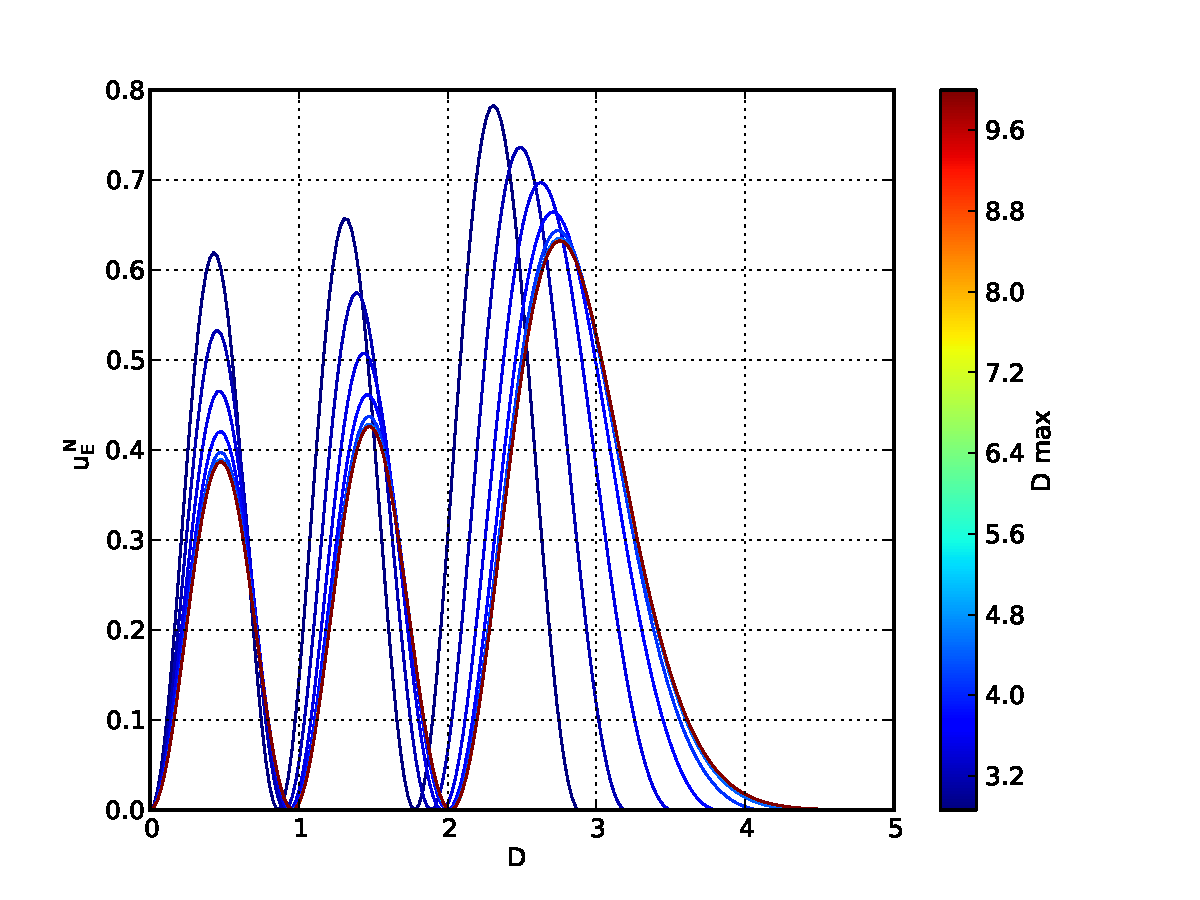
\includegraphics[width=0.81\linewidth]{rhoMaxAnalysis1.pdf}
    \caption{Convergence of the squared wavefunction for the first
        eigenstate of the harmonic oscillator as a function of $\rhomax$
    for $N=200$. The solutions have converged for $\rhomax > 4$.}
    \label{fig:rhoMax1}
\end{figure}

\begin{figure}[H]
    \centering
    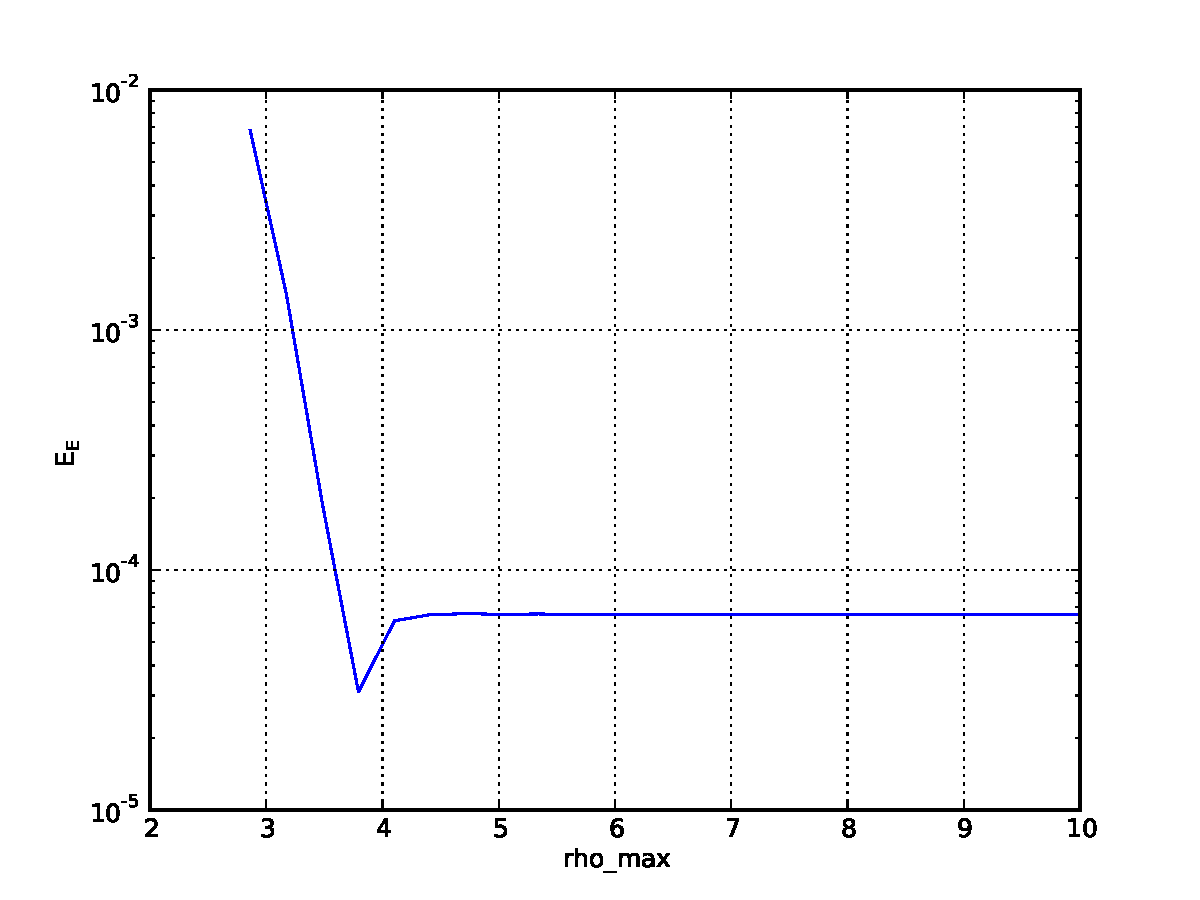
\includegraphics[width=0.81\linewidth]{rhoMaxAnalysis2.pdf}
    \caption{Convergence of the relative error of the first three
        eigenvalues of the 3D harmonic oscillator for increasing $\rhomax$,
        with constant step size $h$. For values above $\rhomax = 5$, no
    improvement is made.}
    \label{fig:rhoMax2}
\end{figure}


\begin{figure}[H]
    \centering
    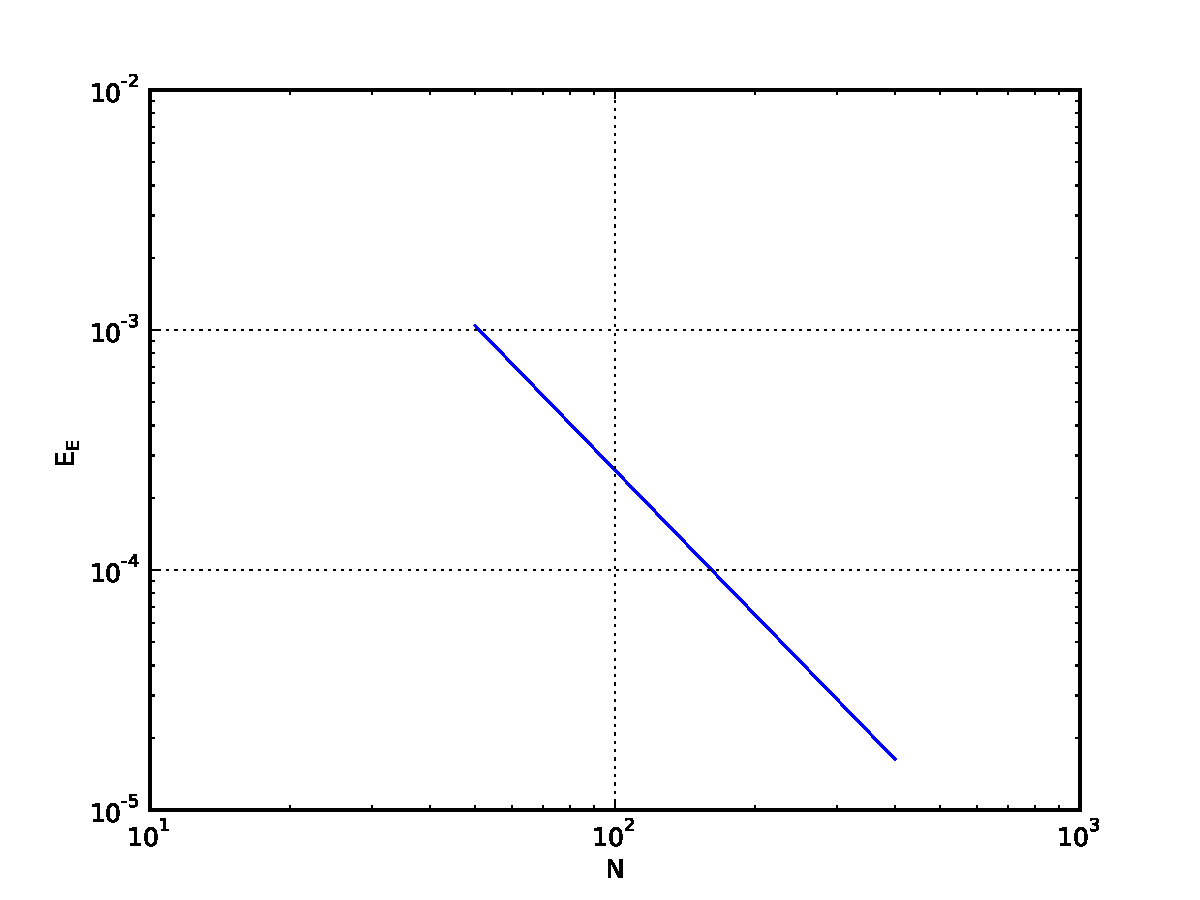
\includegraphics[width=0.85\linewidth]{dimAnalysis2.pdf}
    \caption{Relative error of the three first eigenvalues of the
    non-interacting harmonic oscillator as a function of $N$. $N=200$
produces relative error $\epsilon_i < 10^-4$ for all $i\in{1,2,3}$. The
average gradient of the three functions are $-1.81, -1.67$ and $ -1,60$
respectively.} 
    \label{fig:dim2}
\end{figure}

\subsubsection{Iterations}
Naively one can predict that the number of uses of the rotation algorithm
increases with the amount of matrix elements, $\bigO{N^2}$.
The results \Cref{fig:iterations} verifies this, showing a dependence of
$\bigO{N^{2.06}}$.



\begin{figure}[H]
    \centering
    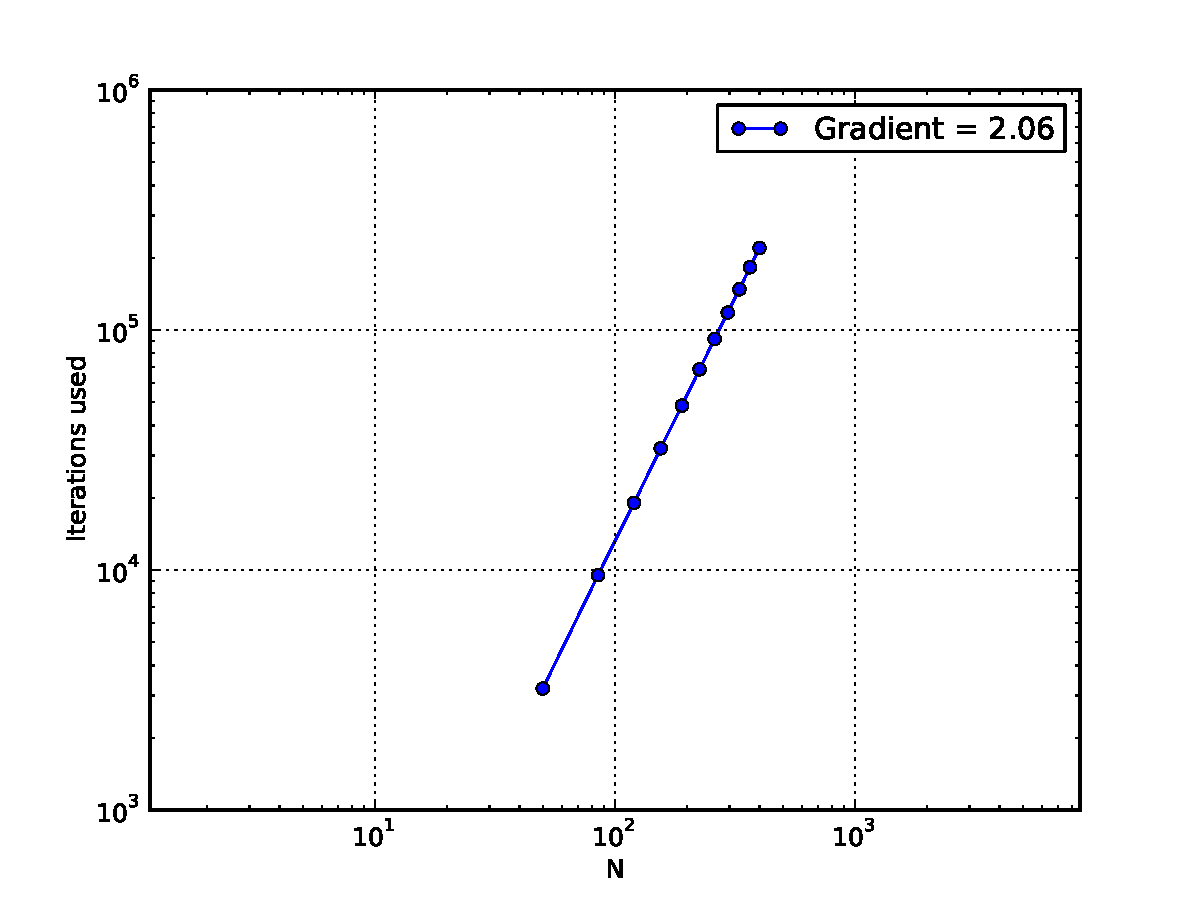
\includegraphics[width=0.83\linewidth]{iterations.pdf}
    \caption{Log-log plot of iterations of jacobi rotate used for the
        Jacobis method to produce a diagonalized (within a certain
        tolerance) matrix, as a function of $N$. The slope in the log plot
        is $2.06$, corresponding to a $\bigO{N^{2.06}}$ dependence.}
    \label{fig:iterations}
\end{figure}


\subsection{Interacting case}
The normalised wave function as a function of the relative coordinate between
electrons in the harmonic oscillator can be seen in \cref{fig:waveFunc}.
A larger value of $\omega_r$ causes a higher electron density. We got the
following three first eigenvalues for the electron:


\begin{center}
\begin{tabular}{ | c | c | c | c | }
    \hline
    $\omega_r$&$E_1$&$E_2$&$E_3$     \\
    $1/10$ & $0.106$ & $0.142$ & $0.178$ \\
    $1/4$ & $1.250$ & $2.190$ & $3.150$ \\
    $1/2$ & $2.230$ & $4.134$ & $6.074$ \\
    $1$ & $4.058$ & $7.909$ & $11.819$\\
    $5$ & $17.448$ & $37.070$ & $56.850$ \\
    \hline
 \end{tabular}
\end{center}




\begin{figure}[H]
    \centering
    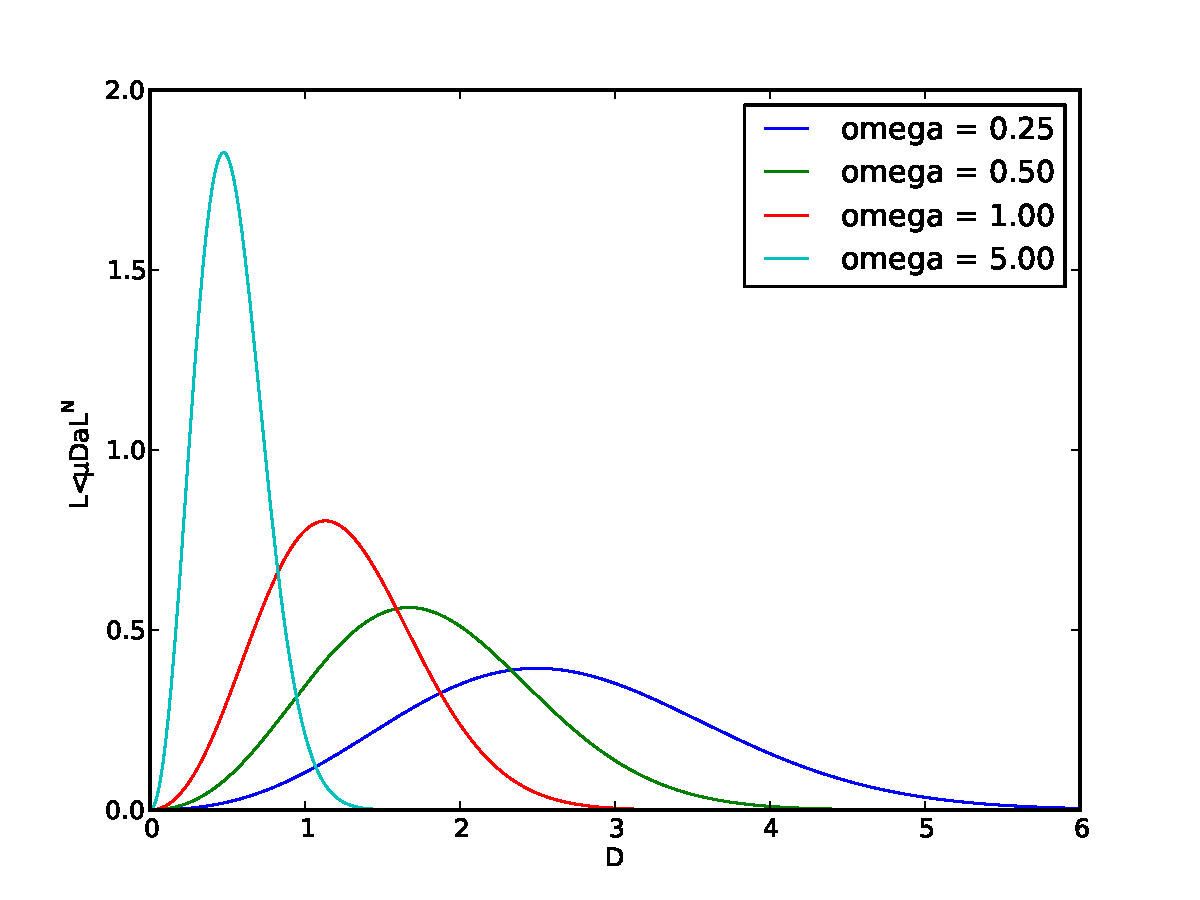
\includegraphics[width=0.85\linewidth]{waveFunc.pdf}
    \caption{The normalised wave functions of the relative coordinate for two
    interacting electrons, for the given $\omega_r$. The lowest value 
$\omega = 0.01$ stretched the wave function too much; it didn't even fit our
plot. One can see that the low energy bound states are spread out more for weak
potentials. }
    \label{fig:waveFunc}
\end{figure}





\section*{Conclusions}
\input{conclusions.tex}
\section*{References}


\end{document}
